When compiling all this data, it is recomended to use python to make repeating your work easier and 
to keep track of the values of variables. 
\\
\\
Because we are using the temperature determination method of color temperature, we have two distinct 
distance values, the B-Filter distance and the V-Filter distance. We will also be determining the line 
of best fit in two different ways, one way with a set y-intercept of 0 and one without a set y-intercept,
giving us another set of B and V filter distances.
\begin{figure} [h!]
    \begin{center}
    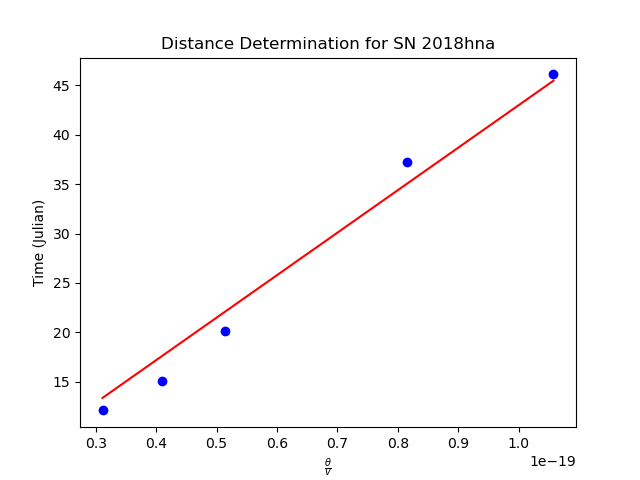
\includegraphics[width=0.5\textwidth]{Distance_Graph.png}
    \end{center}
    \label{fig:distance_graph}
    \caption{The graph of data points in blue and line of best fit in red.}    
\end{figure}
Here is the graph of my data again, with the line of best fit and all the data points available. 
This particular graph is of the V Filter with a Y-Intercept of 0.
\\
\\
Here is a table of the distances calculated with the data collected in previous sections.
\begin{table}[htbp]
    \caption{Distances}
    \label{tab:distances}
    \centering
    \begin{tabular}{|c|c|c|}\hline
    Y-Intercept & Filter Used & Distance (Mpc)\\\hline
    \textit{Standard} & B Filter & 16.37\\
    \textit{} & V Filter & 15.33\\\hline
    \textit{Forced Zero} & B Filter & 14.88\\
    \textit{} & V Filter & 13.93\\\hline
    \end{tabular}
\end{table}
\\
\\
You can see from the determined distances in the table\ref{tab:distances} above that the B Filter generally had a greater distance than the V Filter,
and the forced zero y-intercept reduced the distance as well. These numbers match what other papers have found for this same supernova, 
so we are confident in the accuracy of our answers.
